\chapter{Introduction}
\label{cha:introduction}

The recent development in the deep learning area has resulted in a significant increase in usage of artificial intelligence solutions. Recommendation algorithms, voice or face recognition, type hinting - these are only examples of technologies which are used on a everyday basis by millions. Deep Artificial Neural Networks are by far, the most robust of all machine learning algorithms capable of handling various tasks in an unprecedented manner. Thus I decided to get my hands on designing and implementing vision system for an autonomous boat which uses their full potential.

\section{Real-life applications of Reinforcement Learning}
\label{sec:real-life-applications-of-deep-learning}

\subsection{Games}
\label{sub:intro-games}
RN nowadays is well-known due to algorithm which used to solve different games and managed to achieve a super-human performance in some.
The DQN agent designed by \emph{Google Deep Mind} was able to play 49 different Atari 2600 games (\ref{fig:Atari2600}). However, the most famous one is probably the \emph{AlphaGo} \cite{AlphaGO}  and \emph{AlphaGo Zero}. AlphaGo was trained on countless human games achieving robust performance, but it was not sufficient for the researchers. They let their new agent trained from scratch - AlphaGo Zero to play with itself and eventually beat AlphaGo 100-0. 

\begin{figure}[h]
    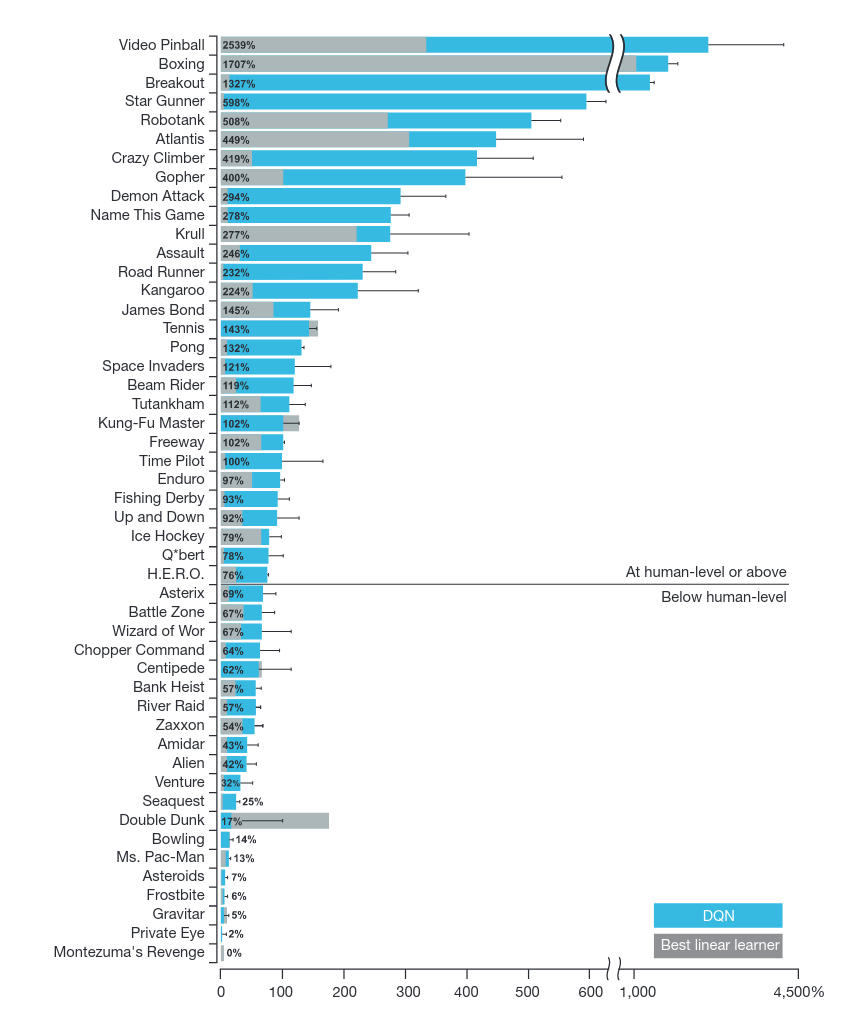
\includegraphics[width=12cm]{img/Atari2600.png}
    \centering
    \caption{Reinforcement Learning model vs human-level performance in the Atari 2600 environment \cite{DQNAtari}}
    \label{fig:Atari2600}
\end{figure}

\subsection{Robotics}
\label{sub:intro-robotics}
As stated in survey \cite{RNSurvey}, \emph{reinforcement learning offers to a robotics a framework and set of tools for the design of sophisticated and hard-to-engineer behaviors}. In fact, these are most of existing ones in a real world. Instead of engineering a set of deterministic movements of a robot in a controlled environment, identical or improved result can be achieved through training in a well-defined task which provides feedback measuring robot's performance. Such approach enables to train robots for performing tasks in more real world environments which are not usually fully controllable. 

\subsection{Personalized Recommendations}
\label{sub:intro-personalized-reccomendations}
News recommendation tends to be challenging due to the fact that most of the users easily get bored. Even if one clicks at the article, there is a low likelihood that it will be read to the end. Therefore Click Through Rate, which is used by many algorithms, standalone is an ineffective indicator. In order to improve the quality of recommendations and address this issue, the DQN was designed and described in \emph{DRN: A Deep Reinforcement Learning Framework for News Recommendation} \cite{DRNNewsRecommendaiton}. This method uses multiple features to determine what will be displayed to the user.

\newpage
\section{Reinforcement Learning Methods Taxonomy}
\label{sec:classification-of-reinforcement-learning-methods}

\subsection{Policy}
\label{sub:policy}

The policy is a strategy used by the agent to achieve desired goal. It dictates which action is going to be taken based on agent's state and the environment. Formally the policy $\pi(s)$, $s\in{S}$, is defined in terms of the \emph{Markov Decision Process} to which it refers. Markov Decision Process can be expressed as a tuple $(S, A, P_a, R_a)$ where:

\begin{itemize}
    \item $S$ is a state space, a set of all possible states of the agents,
    \item $A$ is an action space, a set of all the behaviors agent can take,
    \item $P_a(s, s') = P(s_{t+1} = s' | s_t = s, a_t = a)$ is the probability that the outcome of an action $a$ taken in state $s$ will be state $s'$ at time $t+1$,
    \item $R_a(s, s')$ is the reward received after transition from state $s$ to state $s'$ after taking action $a$.
\end{itemize}

\subsubsection*{Off-Policy}
\label{sub2:off-poicy}

% TODO: Q-value reference
% TODO: Q-learning referece
In an off-policy algorithm the agent state and the action that will be taken is evaluated regardless of the currently followed policy $\pi$. Q-learning is an example. It updates its Q-values using Q-value of the next state $s'$ and the greedy action $a'$. That is, the return for state-action pairs is estimated assuming that a greedy policy was followed even though the agent is not following the greedy policy.

\subsubsection*{On-Policy}
\label{sub2:on-policy}

On the other hand, an on-policy algorithm evaluates which action agent should take with respect to the policy it follows. For example, SARSA is an algorithm which updates its Q-values using Q-value of the next state $s'$ and the current policy's action $a''$. The return for state-action pairs is estimated assuming that the current policy is followed in the next state.

\subsection{Model}
\label{sub:model}

Model is in simple terms the behaviour of an environment. Based on whether the agent needs to know such model to determine a policy RN algorithms can be classified to two groups. There are two main types of networks regarding the model.

\subsubsection*{Model-Free}
\label{sub2:model-free}

A model-free algorithm does not have to learn the model to evaluate its policy. One of the most common examples is \emph{Q-learning}, but such approach is also used in \emph{Actor-critic} or \emph{Policy gradient} methods which search directly over policy space to find policies that result in a better reward from the environment.

\subsubsection*{Model-Based}
\label{sub2:model-based}

A model based algorithm must know the model of an environment before finding an optimal policy. Therefore a value of the next step can be predicted without actually performing that step. \mbox{AlphaGO} (\ref{sub:intro-games}) is an perfect example.

\subsection{Base}
\label{sub:base}

This \textbf{Value-based} network does not store explicitly the policy. Instead, it keeps track only of a value function. The policy can be derived directly from the value function, which means taking an action which corresponds to the best value.
The opposite approach is taken in \textbf{Policy-based} methods, where the representation of the policy $\pi(s)$ is created explicitly and kept in memory during the learning process. 
